% The next command tells RStudio to do "Compile PDF" on book.Rnw,
% instead of this chapter, thereby eliminating the need to switch back to book.Rnw 
% before making the book.
%!TEX root = ../LightingPaper2020.Rnw

%%%%%%%%%%%%%%%%%%%%%%%%%%%%%%%%%%%%%%%%%%%%%%%%%%%%%%%%%%%%%%
\section{Application to non-light EM radiation}
\label{sec:non_light}
%%%%%%%%%%%%%%%%%%%%%%%%%%%%%%%%%%%%%%%%%%%%%%%%%%%%%%%%%%%%%%
  
**** Zeke add a section here on non-light EM radiation. ****





%++++++++++++++++++++++++++++++
\subsection{appendix subsection 1}
\label{sec:appendix_subsection_1}
%++++++++++++++++++++++++++++++
  
% The appendix is an optional section that can contain 
% details and data supplemental to the main text. 
% For example, explanations of experimental details 
% that would disrupt the flow of the main text, but 
% nonetheless remain crucial to understanding and reproducing the research shown; 
% figures of replicates for experiments 
% of which representative data is shown in the main text 
% can be added here if brief, or as Supplementary data. 
% Mathematical proofs of results not central to the paper can be added as an appendix.


%++++++++++++++++++++++++++++++
\subsection{appdendix subsection 2}
\label{sec:appendix_subsection_2}
%++++++++++++++++++++++++++++++
  
\subsection{Nomenclature for meeting 22/06/2020}
  
Radiant power; $\dot{Q}_{em}$ or $\dot{Q}_e$:

\begin{equation}
  \dot{Q}_{em} = \int \dot{Q}_{em, \lambda} \mathrm{d}\lambda \; .
\end{equation}

Other option; $\Phi_{e}$:

\begin{equation}
  \Phi_{e} = \int \Phi_{e, \lambda} \mathrm{d}\lambda \; .
\end{equation}

For the "wrong" radiant power and spectral radiant power as measured by the spectrometer we could use a ': $Q_{em}'$ or $\Phi_{e}'$; and $Q_{em, \lambda}'$ or $\Phi_{e, \lambda}'$.


Weighted radiant power $L_{f_\lambda}$, weighted by a weighting function $f_\lambda$:

\begin{equation}
  \dot{L}_{f_{\lambda}} = \int \dot{Q}_{em, \lambda} f_{\lambda} \mathrm{d}\lambda \; .
\end{equation}

\begin{equation}
  \dot{L}_{V_{\lambda}} = \int \dot{Q}_{em, \lambda} V_{\lambda} \mathrm{d}\lambda \; .
\end{equation}

\begin{equation}
  \dot{L}_{f_{univ, \lambda}} = \int \dot{Q}_{em, \lambda} f_{univ, \lambda} \mathrm{d}\lambda \; .
\end{equation}


Luminous "flux" (or luminous "power") (in lm/Watt):

\begin{equation}
  \Phi_{v} = 683 lm/W \int \dot{Q}_{em, \lambda} V_{\lambda} \mathrm{d}\lambda \; .
\end{equation}


Regarding efficiencies (electricity to light, electricity to radiant power, and radiant power to light):

\begin{figure}
\centering
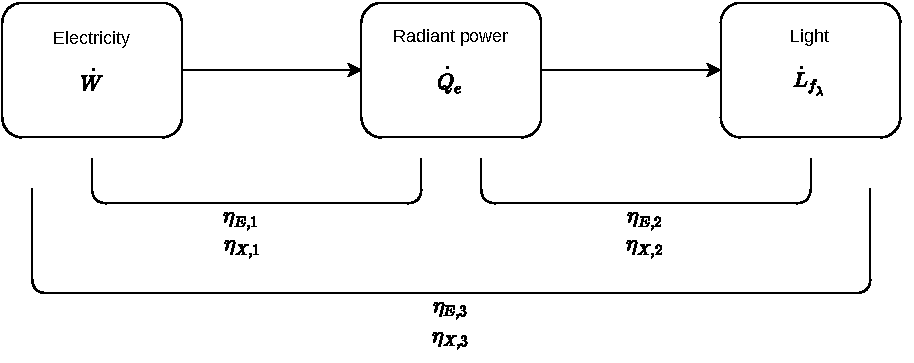
\includegraphics[width=1\linewidth]{figure_other/elec_to_light.pdf}
\caption{Efficiencies in the electricity-to-light conversion}
\end{figure}


% All appendix sections must be cited in the main text. 
% In the appendixes, Figures, Tables, etc. should be labeled starting with `A', 
% e.g., Figure A1, Figure A2, etc. 
